%% MemGate --- IEEE conference paper
%% Compile: pdflatex main / bibtex main / pdflatex main / pdflatex main
%% Numeric tables in tables/ are GENERATED by make_tables.py; do not edit them.
\documentclass[conference]{IEEEtran}
\IEEEoverridecommandlockouts

\usepackage{cite}
\usepackage{amsmath,amssymb}
\usepackage{graphicx}
\usepackage{booktabs}
\usepackage{url}
\usepackage[hidelinks]{hyperref}

\begin{document}

\title{Selection Beats Compression: Memory Decision\\Policies for LLM Agents Under a Bounded Store}

\author{
\IEEEauthorblockN{Simar Singh Khanuja}
\IEEEauthorblockA{\textit{Dept. of Computer Science and Engineering}\\
\textit{SVKM's NMIMS, Indore Campus}\\
Indore, India}
\and
\IEEEauthorblockN{Yash Ramchandani}
\IEEEauthorblockA{\textit{Dept. of Computer Science and Engineering}\\
\textit{SVKM's NMIMS, Indore Campus}\\
Indore, India}
}

\maketitle

\begin{abstract}
A long-running LLM agent cannot keep every turn of a conversation in its
context window, so a memory layer has to decide what to keep, what to compress,
what to forget and what to recall. Tiered memory systems that make these
decisions are already in use, but the decision policy itself has rarely been
isolated and measured. This paper presents MemGate, an evaluation harness that
places competing memory policies on a common accuracy-per-token frontier. Each
comparison is set up so that only one factor differs between the two arms. We
first show that the accounting normally used in this area, which bounds the
context assembled per query but leaves the store unbounded, charges a
store-everything baseline nothing for retention and therefore settles the
comparison in advance. When the store is also bounded, choosing which turns to
forget is worth $+8.67$ answer-recall points over forgetting oldest-first at
identical storage, fidelity and retrieval (95\% CI $[+4.77, +14.27]$ clustered
by conversation, McNemar $p=1.1\!\times\!10^{-4}$), while compressing an evicted
turn instead of dropping it loses $6.71$ points. We also test the
rate--distortion prediction that compression must eventually win. Up to a
compression ratio of $182\times$ it does not, and the margin in favour of
selection widens. Charging the budget for the embedding index, which is
normally left out, reverses the ranking below about 40\,KiB, where a policy
that stores no index at all performs best. Finally, an LLM-judged salience
scorer performs worse than a regular-expression heuristic by $5.87$ points,
with the confidence interval excluding zero. We also report three measurement
errors that changed our own results, each found by an invariant rather than by
inspection.
\end{abstract}

\begin{IEEEkeywords}
large language models, agent memory, context management, retrieval-augmented
generation, rate--distortion, empirical evaluation
\end{IEEEkeywords}

%% ======================================================================
\section{Introduction}
%% ======================================================================

A conversational agent that runs for weeks builds up a history far larger than
any context window, so some component must decide what goes into the prompt on
each turn. Simply using a longer window does not remove the problem. Accuracy
has been shown to fall by 30--50\% well before the documented context limit
across a range of frontier models \cite{chroma2025contextrot}, and the position
of information inside a long context changes how much of it the model actually
uses \cite{liu2024lostmiddle}. These are properties of attention over long
inputs rather than gaps in training, so a larger window moves the difficulty
instead of solving it. The limiting factor is curation rather than capacity.

The cost of poor curation can be measured. On LongMemEval, oracle retrieval
scores about 92\% where the same model retrieving for itself scores about 58\%
\cite{wu2024longmemeval}. The model answers correctly once the right evidence
is placed in front of it, so this 34-point difference is a selection failure
rather than a reasoning failure.

Systems that address selection already exist. Tiered memory with summarisation
and forgetting is used in MemGPT \cite{packer2023memgpt}, MemoryBank
\cite{zhong2024memorybank} and the architectures reviewed in
\cite{zhang2024memorysurvey}. What has not been established is whether the
individual mechanisms inside those systems earn their cost, since they are
evaluated as complete systems rather than as separate decisions. A recent
survey states the gap directly: current systems ``do not solve the fundamental
challenge: deciding what to remember and what to forget''
\cite{zhang2024memorysurvey}. A rate--distortion framing has been proposed for
this family of decisions \cite{colaco2026rd}, but it provides an analytical
framework rather than a measured system.

This paper measures the decision. Our research question is: how much of the
memory-selection gap can a better decision policy recover, and under what
budget does compression become worthwhile? The contributions are as follows.

\begin{enumerate}
\item A storage-budgeted evaluation protocol that corrects an accounting error
common in this area. Bounding only the assembled context charges a
store-everything baseline nothing for retention, so forgetting can only lose
information and the comparison is settled before it is run
(Section~\ref{sec:accounting}).

\item Evidence that the gain comes from selection rather than compression. At
identical storage, fidelity and retrieval, scored forgetting is worth $+8.67$
answer-recall points over FIFO, while compressing an evicted turn loses $6.71$
points (Sections~\ref{sec:selection} and~\ref{sec:significance}).

\item A test of the rate--distortion crossover at which compression should
begin to pay, carried out to a compression ratio of $182\times$
(Section~\ref{sec:scaling}).

\item Byte-denominated accounting, which shows that the embedding index
outweighs the text it indexes by about $12\times$ and reverses the ranking of
policies below roughly 40\,KiB (Section~\ref{sec:bytes}).

\item A negative result for LLM-judged salience. As a single-component swap, a
0.5B instruction-tuned judge performs worse than a hand-written heuristic by
$5.87$ points (Section~\ref{sec:scorer}).

\item Three measurement errors that affected our own results, with the checks
that detected them (Section~\ref{sec:threats}).
\end{enumerate}

Four of these six results are negative or corrective. We consider this a useful
outcome. Described only as a three-tier memory layer, the system would
duplicate work that has already been done; measured against controls, it
indicates which parts of that design actually pay for themselves.

The rest of this paper is organised as follows. Section~\ref{sec:related}
reviews related work. Section~\ref{sec:harness} describes the harness and the
policies it compares, and Section~\ref{sec:metrics} defines the two metrics we
report. Section~\ref{sec:setup} gives the experimental setup and
Section~\ref{sec:results} the results. Section~\ref{sec:threats} discusses
threats to validity, and Sections~\ref{sec:limitations}
and~\ref{sec:conclusion} give limitations and conclusions.

%% ======================================================================
\section{Related Work}
\label{sec:related}
%% ======================================================================

\subsection{Tiered agent memory}
MemGPT \cite{packer2023memgpt} uses an operating-system analogy in which a
virtual context is paged against external storage under the model's own
control. MemoryBank \cite{zhong2024memorybank} adds a forgetting curve derived
from the Ebbinghaus model. Generative Agents \cite{park2023generative} score
memories by recency, importance and relevance before retrieval, and A-MEM
\cite{xu2025amem} organises memories as interlinked notes. This work shows that
tiering and forgetting are practical. Because these systems are evaluated end
to end, however, the contribution of any single decision inside them, such as
what to retain and at what fidelity, cannot be separated from the rest of the
pipeline. Our harness is designed to make that separation possible.

\subsection{Context and cache compression}
A related line of work compresses the prompt or the attention cache instead of
choosing between stored items. LLMLingua \cite{jiang2023llmlingua} prunes
tokens using a perplexity criterion. Gist tokens \cite{mu2023gist} and
AutoCompressors \cite{chevalier2023autocompressor} learn dense summary
representations. StreamingLLM \cite{xiao2024streaming} and
H\textsubscript{2}O \cite{zhang2023h2o} evict entries from the KV cache using
attention-derived scores. All of these operate within a single forward pass
over a contiguous context. The decision studied here is upstream of that and
persistent: it determines which items survive in a store across sessions, where
an evicted item cannot be recovered from the cache at all.

\subsection{Benchmarks}
LoCoMo \cite{maharana2024locomo} provides multi-session dialogues annotated
with gold evidence turn identifiers, which is what allows a retrieval-level
metric to be computed without running a generative model. LongMemEval
\cite{wu2024longmemeval} isolates several memory abilities and is the source of
the oracle-versus-interactive gap quoted above.

\subsection{Position of this work}
We propose neither a new architecture nor a new benchmark. The contribution is
a measurement protocol and the results obtained with it, including a case where
correcting the protocol reverses the conclusion.

%% ======================================================================
\section{The MemGate Harness}
\label{sec:harness}
%% ======================================================================

MemGate is placed between an agent and a frozen LLM, and controls only what
enters the prompt. No component is trained and the base model is treated as a
black box, so any difference we report can be attributed to the memory policy.

\subsection{Tiers as a lifecycle}
The store has three tiers, but they are organised as a lifecycle rather than as
a partition. Every turn enters Tier~1 verbatim, and the routing decision is
taken once, at eviction, when the budget binds. Writing $u$ for the utility
assigned to an item by the scorer:
\[
\begin{array}{ll}
u \geq \tau_{\text{fact}} & \rightarrow\ \text{Tier 3: atomic fact}+\text{vector}\\
u \geq \tau_{\text{low}}  & \rightarrow\ \text{Tier 2: compressed gist}\\
\text{otherwise}          & \rightarrow\ \text{dropped}
\end{array}
\]
Tier~1 holds recent verbatim turns and answers the question \emph{when};
Tier~2 holds compressed gists and answers \emph{gist}; Tier~3 holds durable
facts with embeddings, answers \emph{what}, and enters the context only when
retrieval matches. Scoring each item once, at eviction, is what makes the
decision point separable, since it gives a single site in the pipeline that a
controlled swap can target.

\subsection{Policies}
Table~\ref{tab:policies} lists the arms. Two require comment. RAG is the
no-policy control: it stores everything, retrieves the top $k$ items, and
evicts FIFO when the store is full. It is not a weak baseline but the arm that
a decision policy has to beat in order to have contributed anything. P0 is
given the same token budget as MemGate, so the only difference between them is
which turns are selected, not how many tokens may be spent.

\begin{table}[t]
\caption{Policies compared. P1-A and P1-S differ only in what happens to an
evicted item.}
\label{tab:policies}
\centering
\small
\begin{tabular}{@{}llll@{}}
\toprule
& Policy & Retention rule & Fidelity \\
\midrule
P0     & Sliding window   & recency                & verbatim \\
RAG    & Store-all        & FIFO (\emph{control})  & verbatim \\
P1     & Threshold        & scored at ingest       & compressed \\
P1-A   & Adaptive         & score orders eviction  & \textbf{compress} \\
P1-S   & Select           & score orders eviction  & \textbf{drop} \\
P2     & LLM-judged       & 0.5B model scores turn & drop \\
P3     & Learned          & fitted, cross-validated& drop \\
Oracle & ---              & perfect selection      & verbatim \\
\bottomrule
\end{tabular}
\end{table}

\subsection{One variable per comparison}
The experimental design lies in the set of contrasts rather than in the set of
policies. Each contrast holds everything constant except one factor:

\begin{center}
\small
\begin{tabular}{@{}lll@{}}
\toprule
Contrast & Held constant & Varies \\
\midrule
P0 vs.\ RAG   & retention, storage & read path \\
RAG vs.\ P1-S & storage, fidelity, retrieval & \textbf{what is forgotten} \\
P1-S vs.\ P1-A& storage, selection & \textbf{fidelity} \\
\bottomrule
\end{tabular}
\end{center}

The second contrast is the one this paper depends on. RAG and P1-S hold the
same verbatim turns, in the same embedding space, retrieved by the same
procedure, under the same storage cap. The only difference is which turns are
discarded when the cap binds: oldest-first for RAG, lowest-utility-first for
P1-S. Any gap between the two is therefore attributable to the decision policy.

%% ======================================================================
\section{Metrics}
\label{sec:metrics}
%% ======================================================================

We report two retrieval-level metrics. Evidence recall, also called strict
recall, is the fraction of questions for which every gold evidence turn reached
the assembled context. Answer recall is the fraction for which the answer text
survived into the context, computed over the 715 of 1{,}527 questions whose
answer is literally recoverable from the evidence turns.

The distinction matters for this study. Evidence recall credits an identifier:
a compressed gist retains the evidence identifier of a turn whose text it has
discarded, and so records a hit with none of the answer behind it. During
development we observed evidence recall rise from 8.1\% to 14.8\% while answer
recall remained at 12.8\%, so the apparent gain was entirely an artefact of
identifier bookkeeping. Since the comparison studied here, dropping against
compressing, is the comparison on which the two metrics diverge, reporting only
evidence recall would have produced the opposite conclusion. We therefore treat
answer recall as the primary metric and report evidence recall alongside it so
that the divergence remains visible.

Both metrics are forms of context recall: they measure whether the memory
policy placed the required evidence in front of the model. This is an upper
bound on end-task accuracy rather than accuracy itself, which we return to in
Section~\ref{sec:limitations}. Its advantage for the present study is that it
is deterministic and does not confound the memory policy with the reader's
reasoning ability.

%% ======================================================================
\section{Experimental Setup}
\label{sec:setup}
%% ======================================================================

\subsection{Benchmark}
We use LoCoMo \cite{maharana2024locomo}, which contains 10 multi-session
conversations, 5{,}882 turns and 1{,}527 scoreable questions. Category-5
(adversarial) items are excluded. Those items carry evidence, but the correct
behaviour is for the agent to decline to answer, so retrieving their evidence
would not constitute success.

\subsection{Components}
Retrieval and semantic supersession use all-MiniLM-L6-v2
\cite{reimers2019sbert} with 384 dimensions. Token budgets are counted with the
\texttt{cl100k\_base} tokenizer, so a budget is an exact token count rather
than a word-count approximation. The P2 judge is Qwen2.5-0.5B-Instruct
\cite{qwen2025}, run locally. Salience is read as a continuous expectation over
digit-token logits at a single forward pass, instead of generating a digit and
parsing it. This is faster, cannot produce an output that fails to parse, and gives a
continuous score, so the eviction ranking contains no ties.

\subsection{Statistical procedure}
All intervals are paired bootstrap intervals \cite{efron1993bootstrap} with
$B=10{,}000$ resamples drawn at the conversation level rather than the question
level, reported together with an exact McNemar test \cite{mcnemar1947}. The
choice of resampling unit is not a detail: 1{,}527 questions drawn from 10
conversations are not 1{,}527 independent trials, and one of our own earlier
claims does not survive the correction (Section~\ref{sec:significance}).

\subsection{Reproducibility}
Every model is a pinned local copy and the model hub is disabled when the
package is imported, since a run that can silently download a model is a run
whose inputs are not pinned. All numeric tables in this paper are generated
directly from the committed result files rather than transcribed.

%% ======================================================================
\section{Results}
\label{sec:results}
%% ======================================================================

\subsection{Storage was never budgeted}
\label{sec:accounting}

Experiments in this area cap the context assembled per query and leave the
store unbounded, and our own experiments did the same until this point. Under
that accounting a store-everything baseline is charged nothing for holding all
419 turns of a conversation, so forgetting can only lose information. Run under
those conditions, our own ablation reported the tiering and compression
machinery as a net loss against simply keeping everything and retrieving, and
that result was correct given how the cost was being counted.

Imposing a storage budget $S$ changes the question from what fits in the
context to what is worth keeping at all. Fig.~\ref{fig:frontier} sweeps $S$
with the context budget fixed at 2048 tokens. The ranking under the corrected
accounting differs from the ranking under the original one. This is the most
consequential observation in the paper, because an evaluation protocol that
omits a cost answers a different question from the one it appears to ask.

\begin{figure*}[t]
\centering
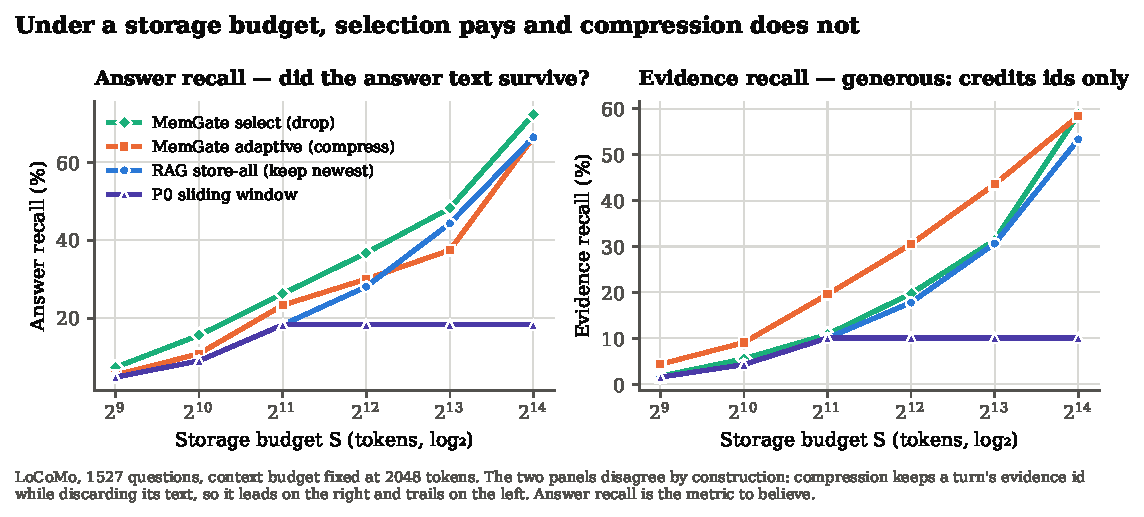
\includegraphics[width=\textwidth]{figures/fig1_storage_frontier.pdf}
\caption{The storage-budget frontier. The context budget is fixed at 2048
tokens and the store is swept. Left: evidence recall. Right: answer recall.
Under evidence recall the compressing policy P1-A appears to lead. Under answer
recall, which checks content rather than identifiers, it does not.}
\label{fig:frontier}
\end{figure*}

\subsection{Selection pays; compression does not}
\label{sec:selection}

Table~\ref{tab:storage} reports both metrics across the sweep. P1-S, which
drops the lowest-utility item when the cap binds, leads on answer recall at
every budget. P1-A, which compresses that item instead of dropping it, leads on
evidence recall at every budget and trails on answer recall, by 6.9 points at
$S=8192$.

This is the identifier problem of Section~\ref{sec:metrics} in practice. A
demoted gist retains the evidence identifiers of a turn whose text has been
discarded. An evaluation reporting only evidence recall would conclude that
compression is the better use of a bounded store, and an evaluation that checks
whether the answer text survived reaches the opposite conclusion.

\begin{table}[t]
\caption{Recall against the storage budget $S$ in tokens, with the context
budget fixed at 2048. $\Delta$ is P1-S minus RAG on answer recall: identical
storage, identical fidelity, identical retrieval, differing only in which turns
are forgotten.}
\label{tab:storage}
\centering
\small
% GENERATED by paper/make_tables.py -- do not edit by hand.
\begin{tabular}{@{}rrrrrrrr@{}}
\toprule
& \multicolumn{3}{c}{Evidence recall (\%)} & \multicolumn{3}{c}{Answer recall (\%)} & \\
\cmidrule(lr){2-4}\cmidrule(lr){5-7}
$S$ & RAG & P1-A & P1-S & RAG & P1-A & P1-S & $\Delta$ \\
\midrule
1024 & 4.3 & 9.1 & 5.6 & 9.1 & 10.9 & \textbf{15.7} & \textbf{$+6.6$} \\
2048 & 10.1 & 19.6 & 10.9 & 18.3 & 23.4 & \textbf{26.3} & \textbf{$+8.0$} \\
4096 & 17.8 & 30.5 & 19.8 & 28.1 & 30.1 & \textbf{36.8} & \textbf{$+8.7$} \\
8192 & 30.6 & 43.5 & 31.4 & 44.3 & 37.5 & \textbf{48.2} & \textbf{$+3.9$} \\
16384 & 53.3 & 58.4 & 58.7 & 66.4 & 66.4 & \textbf{72.3} & \textbf{$+5.9$} \\
\bottomrule
\end{tabular}

\end{table}

\subsection{Statistical significance}
\label{sec:significance}

Table~\ref{tab:significance} reports each contrast with intervals resampled at
the conversation level. The answer-recall gain of scored eviction over FIFO is
$+8.67$ points with the interval excluding zero. The corresponding
evidence-recall gain is $+1.96$ points and does not survive clustering
($p=0.16$), so we do not claim it. We report it here rather than omitting it,
since a claim that fails a correctness check is itself information about the
check.

The P1-S against P1-A rows show the divergence with signs attached: $+6.71$ on
answer recall and $-10.74$ on evidence recall, both significant. The two
metrics therefore disagree in direction and not only in magnitude.

\begin{table*}[t]
\caption{Paired bootstrap ($B=10{,}000$) resampled by conversation, with exact
McNemar, at $S=4096$. The second row is the claim we decline to make.}
\label{tab:significance}
\centering
\small
% GENERATED by paper/make_tables.py -- do not edit by hand.
\begin{tabular}{@{}llrcrc@{}}
\toprule
Comparison & Metric & $\Delta$ (pts) & 95\% CI (clustered) & McNemar $p$ & \\
\midrule
P1-S vs.\ RAG (FIFO) & answer & \textbf{$+8.67$} & $[+4.77,\, +14.27]$ & $1.1\!\times\!10^{-4}$ & $\checkmark$ \\
P1-S vs.\ RAG (FIFO) & evidence & $+1.96$ & $[-1.48,\, +5.52]$ & 0.16 & \textsc{n.s.} \\
P1-S vs.\ P1-A (compress) & answer & \textbf{$+6.71$} & $[+4.24,\, +9.54]$ & $3.6\!\times\!10^{-5}$ & $\checkmark$ \\
P1-S vs.\ P1-A (compress) & evidence & \textbf{$-10.74$} & $[-13.65,\, -7.90]$ & $4.7\!\times\!10^{-20}$ & $\checkmark$ \\
P1-S vs.\ P0 (recency) & answer & \textbf{$+18.46$} & $[+14.68,\, +23.56]$ & $3.8\!\times\!10^{-17}$ & $\checkmark$ \\
P1-S vs.\ P0 (recency) & evidence & \textbf{$+9.69$} & $[+6.85,\, +12.83]$ & $3.6\!\times\!10^{-14}$ & $\checkmark$ \\
\bottomrule
\end{tabular}

\end{table*}

\subsection{The rate--distortion crossover is not reached}
\label{sec:scaling}

Rate--distortion reasoning predicts that compression must eventually beat
selection, since a sufficiently compressed record of everything should
outperform a faithful record of a subset \cite{colaco2026rd}. Sweeping $S$
downward cannot test this prediction, because all policies reach the floor
before any crossover can appear: at $S=256$ every policy sits near 0.2\%
evidence recall.

The axis that is missing is conversation length. We therefore concatenate up to
ten LoCoMo conversations, giving 186K tokens, and hold $S$ fixed, which raises
the compression ratio to $182\times$. Table~\ref{tab:scaling} and
Fig.~\ref{fig:scaling} report the outcome. No crossover occurs, and the margin
of selection over compression does not close. At this scale the best operating
point is at the vertex of the trade-off, where a subset held at full fidelity
outperforms everything held at reduced fidelity.

One caveat applies. A concatenated stream is not a natural long conversation.
Each question concerns one of the constituent conversations, so the others act
as distractors. The experiment is therefore a stress test of retention under
pressure, which is the variable under study, rather than a long-dialogue
benchmark. The negative result is correspondingly bounded: we falsify the
crossover on this axis and up to this ratio, and do not claim that it cannot
occur elsewhere.

\begin{table}[t]
\caption{Answer recall against compression ratio at $S=2048$. The rightmost
column is the margin of dropping over compressing.}
\label{tab:scaling}
\centering
\small
% GENERATED by paper/make_tables.py -- do not edit by hand.
\begin{tabular}{@{}rrrrr@{}}
\toprule
Ratio & RAG & P1-A & P1-S & P1-S $-$ P1-A \\
\midrule
9$\times$ & 18.3 & 23.4 & \textbf{26.3} & $+2.9$ \\
18$\times$ & 10.8 & 14.7 & \textbf{18.2} & $+3.5$ \\
45$\times$ & 7.8 & 11.2 & \textbf{11.7} & $+0.6$ \\
91$\times$ & 4.6 & 6.0 & \textbf{8.7} & $+2.7$ \\
\bottomrule
\end{tabular}

\end{table}

\begin{figure}[t]
\centering
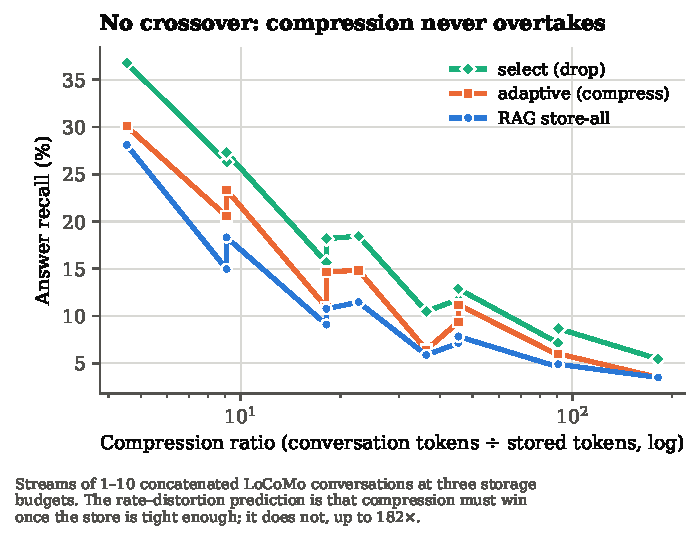
\includegraphics[width=\columnwidth]{figures/fig2_scaling.pdf}
\caption{Compression ratio against answer recall. Theory predicts that the
compressing policy overtakes the selecting one as the ratio grows. Up to
$182\times$ it does not.}
\label{fig:scaling}
\end{figure}

\subsection{The embedding index is not free}
\label{sec:bytes}

Denominating storage in text tokens leaves out the index that makes retrieval
possible. A 384-dimensional \texttt{float32} vector occupies 1{,}536\,B, while
a LoCoMo turn averages about 130\,B of text. The index therefore outweighs the
content it indexes by roughly a factor of 12, and the limiting resource becomes
the number of stored items rather than their length.

Table~\ref{tab:cost} repeats the sweep with the budget denominated in bytes and
each retrievable item charged for its vector. Two results follow. First, the
selection finding of Section~\ref{sec:selection} is robust to the change of
units, since P1-S leads at every budget above 32\,KiB. Second, below
approximately 40\,KiB an embedding index cannot pay for its own storage: P0,
which maintains no index, performs best. A protocol that counts only text
cannot observe this regime, which is the regime that a memory layer on a
constrained device would occupy.

\begin{table}[t]
\caption{Answer recall (\%) with the budget denominated in bytes, charging
1{,}536\,B per retrievable item for its embedding. P0 maintains no index and is
therefore flat.}
\label{tab:cost}
\centering
\small
% GENERATED by paper/make_tables.py -- do not edit by hand.
\begin{tabular}{@{}rrrrr@{}}
\toprule
Budget (KiB) & P0 & RAG & P1-A & P1-S \\
\midrule
32 & \textbf{18.3} & 5.0 & 7.3 & 15.1 \\
64 & 18.3 & 11.0 & 9.4 & \textbf{22.5} \\
128 & 18.3 & 20.0 & 12.3 & \textbf{32.7} \\
256 & 18.3 & 33.0 & 14.3 & \textbf{39.0} \\
512 & 18.3 & 50.3 & 19.2 & \textbf{53.1} \\
\bottomrule
\end{tabular}

\end{table}

\begin{figure}[t]
\centering
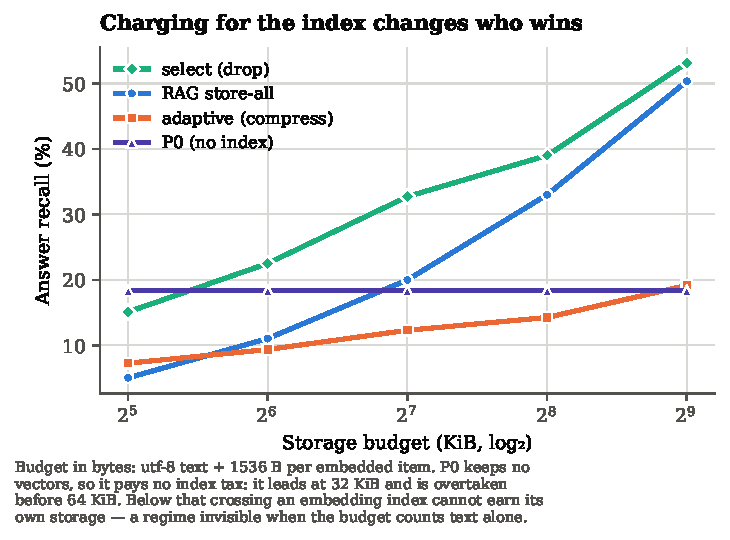
\includegraphics[width=\columnwidth]{figures/fig4_cost_model.pdf}
\caption{Byte-denominated budget. The crossing at the left of the plot is a
policy with no index overtaking every retrieval-based method.}
\label{fig:cost}
\end{figure}

\subsection{Scorer analysis}
\label{sec:scorer}

If the decision is where the value lies, then the scorer that makes it is the
component to improve. Table~\ref{tab:ablation} removes one mechanism at a time.
Retrieval dominates, at $-30.3$ evidence points, and scored eviction is worth
$5.0$ points. The demotion row is marked because it shows the same divergence
in miniature: removing demotion costs $10.7$ evidence points and gains $6.7$
answer points.

\begin{table}[t]
\caption{Component ablation at $S=4096$, showing the change from the full
system. $\dagger$: the row on which the two metrics disagree in direction.}
\label{tab:ablation}
\centering
\small
% GENERATED by paper/make_tables.py -- do not edit by hand.
\begin{tabular}{@{}lrr@{}}
\toprule
Component removed & $\Delta$ evidence & $\Delta$ answer \\
\midrule
Retrieval (Tier 3) & $-30.3$ & $-27.7$ \\
Demotion on pressure\,$\dagger$ & $-10.7$ & $+6.7$ \\
Scored eviction ($\rightarrow$ FIFO) & $-5.0$ & $-6.7$ \\
Informative compressor & $-3.8$ & $-2.2$ \\
Consolidation merge & $-2.6$ & $-5.0$ \\
Semantic supersession & $-0.2$ & $-0.1$ \\
\bottomrule
\end{tabular}

\end{table}

Table~\ref{tab:scorers} varies only the scorer, with the policy, storage
budget, retrieval and compression fixed at the configuration of
Section~\ref{sec:selection}, so any change can be attributed to the scorer.
Three observations follow, all significant under clustering.

First, scoring is worth doing at all. The hand-written heuristic gains $+11.19$
answer points over unscored recency. This row establishes that the decision
point is where value can be added, without which the rest of the table would
not be informative.

Second, the LLM judge still performs worse. Qwen2.5-0.5B-Instruct reaches
30.9\% against the heuristic's 36.8\%, a difference of $-5.87$ points with the
interval excluding zero, at roughly fifteen minutes of GPU time per corpus
against microseconds for a regular expression. This is a negative result rather
than an inconclusive one.

Third, the headroom is real. A logistic scorer fitted under
leave-one-conversation-out, so that the model scoring a conversation never saw
it during training, reaches 48.3\%, which is $+11.47$ over the heuristic. The
judge was therefore not limited by a ceiling that does not exist.

We attribute the judge's failure to what it is shown. It rates each turn in
isolation, and salience is not a property of a turn considered alone: a phone
number is important because a later turn asks for it. The fitted scorer sees
the same isolated text and performs better because it was fitted to which turns
were in fact cited, which lets it absorb corpus-level base rates that a
per-turn prompt cannot convey. Consistent with this, the strongest single
feature recovered by the fitted model is turn length, ahead of every
hand-designed cue, which is a corpus-level regularity rather than a semantic
one.

The fitted scorer is an upper bound and not a deployable component, since a
live agent has no future questions to fit against. Its purpose here is to
bracket what a learned decision policy could achieve.

\begin{table}[t]
\caption{Single-component scorer swap at $S=4096$ with context 2048. Policy,
retrieval and compression are fixed and only the scorer varies. P3 is an upper
bound rather than a deployable component.}
\label{tab:scorers}
\centering
\small
% GENERATED by paper/make_tables.py -- do not edit by hand.
\begin{tabular}{@{}llrrrc@{}}
\toprule
& What the scorer sees & Evid. & Ans. & $\Delta$ vs.\ P1 & 95\% CI \\
\midrule
P0 & position only & 12.6 & 25.6 & $-11.19$ & $[-17.24,\, -6.19]$ \\
P1 & regex + shallow NER & 19.8 & \textbf{36.8} & --- & --- \\
P2 & the turn, in isolation & 14.0 & 30.9 & $-5.87$ & $[-10.77,\, -1.76]$ \\
P3 & turn + fitted base rates & 33.4 & 48.3 & $+11.47$ & $[+4.90,\, +17.86]$ \\
\bottomrule
\end{tabular}

\end{table}

\begin{figure}[t]
\centering
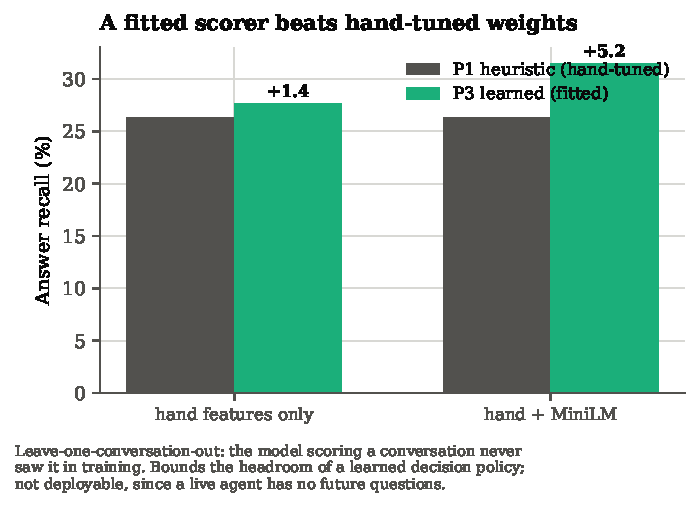
\includegraphics[width=\columnwidth]{figures/fig3_scorer.pdf}
\caption{Scorer comparison. The LLM judge P2 does not reach the heuristic P1,
while the fitted bound P3 shows that headroom is available.}
\label{fig:scorer}
\end{figure}

%% ======================================================================
\section{Threats to Validity}
\label{sec:threats}
%% ======================================================================

Three errors changed our results before we detected them. Each was found by an
invariant rather than by reading the code, and we report them because we
believe they apply to other evaluations of agent memory.

\subsection{A policy that reads its evaluation label}
LoCoMo supplies a \texttt{fact\_id} for each evidence turn. An early
consolidation rule promoted items using that field, so the policy was
consulting the answer key when deciding what to keep. The effect was worth 45
to 47 recall points and invalidated our first reported result. The remedy is an
invariant rather than a coding convention: when every evaluation label is
stripped from the input, the resulting store must be bit-identical. Each
decision point added since, including eviction under a storage budget and
demotion, was placed under that invariant before any number derived from it was
reported.

\subsection{Measured component value depends on the current bottleneck}
We initially measured the sentence embedder as worth $+0.2$ points and
concluded that it barely mattered. That was true in the regime measured, where
retrieval was saturated against a write path that discarded 93\% of the
conversation. After that bottleneck was removed, the same substitution was
worth $+19.7$ points. An ablation run against a bottlenecked pipeline will
systematically undervalue the components that would matter once the bottleneck
moves, which argues for repeating ablations after any change to the dominant
term rather than treating them as settled.

\subsection{A metric that credits identifiers}
This was discussed in Section~\ref{sec:metrics} and is listed again here
because it is a threat to validity and not only a definitional choice. An
identifier-level metric applied to a system that can store identifiers without
their content measures the system's bookkeeping rather than its memory.

A fourth and narrower case is worth recording. Batched judge scoring returned
\texttt{NaN} for the short turns specifically. The natural hypothesis is
numerical precision, and moving to \texttt{float32} did not resolve it. The
cause was left-padding, which produces fully masked attention rows. Without an
explicit \texttt{NaN} guard, every filler turn would have scored \texttt{NaN}
and inverted the eviction order, and the failure would not have been visible in
the aggregate metrics.

%% ======================================================================
\section{Limitations}
\label{sec:limitations}
%% ======================================================================

\emph{Ten conversations.} Clustering by conversation is the correct unit of
analysis and leaves few clusters, so the intervals are wide. We report them,
and report the one effect that does not survive as not significant.

\emph{Context recall is an upper bound.} We measure whether the required
evidence reached the context, not whether the model then answered correctly. An
end-task evaluation through a fixed local reader has been implemented, with a
closed-book floor and an oracle ceiling as controls, but at the time of writing
it has only been validated on a pilot too small to support a claim. We
therefore report no end-task accuracy figures here.

\emph{Extractive compression only.} P1-A selects words and does not rewrite
them. Our negative result for compression is stated for the extractive case,
and an abstractive summariser may retain more content per token.

\emph{Concatenated streams are synthetic}, as discussed in
Section~\ref{sec:scaling}.

\emph{Single embedder and single judge.} The negative result of
Section~\ref{sec:scorer} is evidence about a 0.5B model prompted per turn, not
about LLM-judged salience in general. A larger judge, or one shown the
neighbouring turns, remains untested and is the most direct way to challenge
the finding.

%% ======================================================================
\section{Conclusion}
\label{sec:conclusion}
%% ======================================================================

Under the accounting normally used in this area, tiered compression is a net
loss against storing everything and retrieving, but that result is an artefact
of leaving the store unbounded. When the store is bounded, the decision of
which items to forget is worth $+8.67$ answer-recall points at identical
storage, fidelity and retrieval, while compressing an evicted item rather than
dropping it loses $6.71$ points. The crossover at which compression should
begin to pay is not reached on this benchmark up to a compression ratio of
$182\times$. Charging the budget for the embedding index reverses the ranking
of policies below about 40\,KiB. An LLM judge, which is the obvious route to a
better scorer, performs worse than a regular expression, and the reason can be
identified: salience is not a property of a turn considered in isolation.

The practical recommendation is narrow. Retain a scored subset at full fidelity
rather than compressing everything, and denominate the budget in bytes with the
index included. The methodological recommendation is broader. Three of the
results above changed in sign or in magnitude once a measurement error was
removed, and none of those errors was visible in the aggregate numbers they
affected.

Future work follows directly from the limitations. The end-task evaluation
needs to be completed at full scale. Abstractive compression would test whether
the negative result is specific to extractive methods. A benchmark with
genuinely long single conversations, such as LongMemEval, would replace the
concatenated-stream stress test. Finally, learning the eviction policy online
would remove the dependence on future questions that makes the fitted scorer an
upper bound rather than a usable component.

\section*{Acknowledgment}
The authors thank the faculty of SVKM's NMIMS, Indore Campus, for their
guidance throughout this capstone project.

\bibliographystyle{IEEEtran}
\bibliography{refs}

\end{document}
